\documentclass[a4paper,12pt]{article}
\usepackage[utf8]{inputenc}
\usepackage[T2A]{fontenc}
\usepackage[russian]{babel}
\usepackage{amsmath, amssymb, amsfonts, amsthm}
\usepackage{graphicx}
\usepackage{geometry}
\usepackage{float}
\usepackage[hidelinks, pdfencoding=auto, psdextra]{hyperref}
\usepackage{tocloft}
\usepackage{fancyhdr}
\usepackage{enumitem}
\usepackage{listings}
\usepackage{xcolor}
\usepackage{subcaption}

\geometry{top=2cm, bottom=2cm, left=2.5cm, right=2cm}
\setlength{\headheight}{14.5pt}

\begin{document}

\begin{titlepage}
    \centering
    {\Large \bfseries Федеральное государственное автономное образовательное учреждение высшего образования «Национальный исследовательский университет ИТМО» \par}
    
    {\large Факультет программной инженерии и компьютерной техники \par}
    \vspace{2cm}
    {\LARGE Домашнее задание №2 \par}
    \vspace{0.5cm}
    {\Large Вариант 74 \par}
    \vspace{2cm}
    \vfill
    \begin{flushright}
        \large
        \textbf{Выполнил:} \\
        Шулай Роман \\
        Группа P3115 \\
        \vspace{1cm}
        \textbf{Преподаватель:} \\
        Поляков Владимир Иванович \\
    \end{flushright}
    \vfill
    {\large Санкт-Петербург \\ 2026 год}
\end{titlepage}
\newpage
\setcounter{page}{2}

\begin{figure}[htbp]
    \centering
    \begin{subfigure}[b]{0.45\textwidth}
        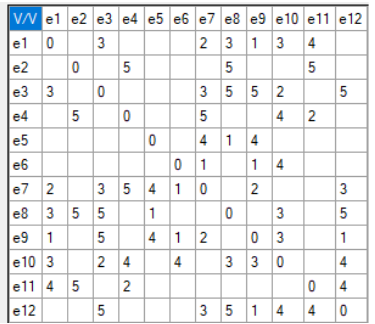
\includegraphics[width=\linewidth]{images/matrix.png}
        \caption{Матрица смежности}
        \label{fig:sub1}
    \end{subfigure}
    \hfill % Распорка для равномерного распределения
    \begin{subfigure}[b]{0.45\textwidth}
        
\includegraphics[width=\linewidth]{images/graph.png}
        \caption{Граф}
        \label{fig:sub2}
    \end{subfigure}
    %\caption{Общая подпись для двух картинок}
    \label{fig:main}
\end{figure}

\noindent
1. $l(x_1) = 0^+;\ l(x_i) = \infty$ \\
2. Гр = $\{x_{3}, x_{7}, x_{8}, x_{9}, x_{10}, x_{11}\}$ – временные пометки имеют вершины $x_{3}, x_{7}, x_{8}, x_{9}, x_{10}, x_{11}$, уточним их: \\
\indent $l(x_{3}) = min[\infty, 0.0 + 3.0] = 3.0$, \\
\indent $l(x_{7}) = min[\infty, 0.0 + 2.0] = 2.0$, \\
\indent $l(x_{8}) = min[\infty, 0.0 + 3.0] = 3.0$, \\
\indent $l(x_{9}) = min[\infty, 0.0 + 1.0] = 1.0^+$, \\
\indent $l(x_{10}) = min[\infty, 0.0 + 3.0] = 3.0$, \\
\indent $l(x_{11}) = min[\infty, 0.0 + 4.0] = 4.0$ \\
3. Постоянную пометку получает $min[l(x_i)] = l(x_{9}) = 1.0^+$, $p = 9$ \\
4. Гр = $\{x_{1}, x_{3}, x_{5}, x_{6}, x_{7}, x_{10}, x_{12}\}$ – временные пометки имеют вершины $x_{3}, x_{5}, x_{6}, x_{7}, x_{10}, x_{12}$, уточним их: \\
\indent $l(x_{3}) = min[3.0, 1.0 + 5.0] = 3.0$, \\
\indent $l(x_{5}) = min[\infty, 1.0 + 4.0] = 5.0$, \\ 
\indent $l(x_{6}) = min[\infty, 1.0 + 1.0] = 2.0^+$, \\
\indent $l(x_{7}) = min[2.0, 1.0 + 2.0] = 2.0$, \\
\indent $l(x_{10}) = min[3.0, 1.0 + 3.0] = 3.0$, \\
\indent $l(x_{12}) = min[\infty, 1.0 + 1.0] = 2.0$ \\
5. Постоянную пометку получает $min[l(x_i)] = l(x_{6}) = 2.0^+$, $p = 6$ \\
6. Гр = $\{x_{7}, x_{9}, x_{10}\}$ – временные пометки имеют вершины $x_{7}, x_{10}$, уточним их: \\
\indent $l(x_{7}) = min[2.0, 2.0 + 1.0] = 2.0^+$, \\
\indent $l(x_{10}) = min[3.0, 2.0 + 4.0] = 3.0$ \\
7. Постоянную пометку получает $min[l(x_i)] = l(x_{7}) = 2.0^+$, $p = 7$ \\
8. Гр = $\{x_{1}, x_{3}, x_{4}, x_{5}, x_{6}, x_{9}, x_{12}\}$ – временные пометки имеют вершины $x_{3}, x_{4}, x_{5}, x_{12}$, уточним их: \\
\indent $l(x_{3}) = min[3.0, 2.0 + 3.0] = 3.0$, \\
\indent $l(x_{4}) = min[\infty, 2.0 + 5.0] = 7.0$, \\
\indent $l(x_{5}) = min[5.0, 2.0 + 4.0] = 5.0$, \\
\indent $l(x_{12}) = min[2.0, 2.0 + 3.0] = 2.0^+$ \\
9. Постоянную пометку получает $min[l(x_i)] = l(x_{12}) = 2.0^+$, $p = 12$ \\
10. Гр = $\{x_{3}, x_{7}, x_{8}, x_{9}, x_{10}, x_{11}\}$ – временные пометки имеют вершины $x_{3}, x_{8}, x_{10}, x_{11}$, уточним их: \\
\indent $l(x_{3}) = min[3.0, 2.0 + 5.0] = 3.0^+$, \\
\indent $l(x_{8}) = min[3.0, 2.0 + 5.0] = 3.0$, \\
\indent $l(x_{10}) = min[3.0, 2.0 + 4.0] = 3.0$, \\
\indent $l(x_{11}) = min[4.0, 2.0 + 4.0] = 4.0$ \\
11. Постоянную пометку получает $min[l(x_i)] = l(x_{3}) = 3.0^+$, $p = 3$ \\
12. Гр = $\{x_{1}, x_{7}, x_{8}, x_{9}, x_{10}, x_{12}\}$ – временные пометки имеют вершины $x_{8}, x_{10}$, уточним их: \\
\indent $l(x_{8}) = min[3.0, 3.0 + 5.0] = 3.0^+$, \\
\indent $l(x_{10}) = min[3.0, 3.0 + 2.0] = 3.0$ \\
13. Постоянную пометку получает $min[l(x_i)] = l(x_{8}) = 3.0^+$, $p = 8$ \\
14. Гр = $\{x_{1}, x_{2}, x_{3}, x_{5}, x_{10}, x_{12}\}$ – временные пометки имеют вершины $x_{2}, x_{5}, x_{10}$, уточним их: \\
\indent $l(x_{2}) = min[\infty, 3.0 + 5.0] = 8.0$, \\
\indent $l(x_{5}) = min[5.0, 3.0 + 1.0] = 4.0$, \\
\indent $l(x_{10}) = min[3.0, 3.0 + 3.0] = 3.0^+$ \\
15. Постоянную пометку получает $min[l(x_i)] = l(x_{10}) = 3.0^+$, $p = 10$ \\
16. Гр = $\{x_{1}, x_{3}, x_{4}, x_{6}, x_{8}, x_{9}, x_{12}\}$ – временные пометки имеют вершины $x_{4}$, уточним их: \\
\indent $l(x_{4}) = min[7.0, 3.0 + 4.0] = 7.0$ \\
17. Постоянную пометку получает $min[l(x_i)] = l(x_{5}) = 4.0^+$, $p = 5$ \\
18. Гр = $\{x_{7}, x_{8}, x_{9}\}$ – все вершины имеют постоянные пометки. \\
19. Постоянную пометку получает $min[l(x_i)] = l(x_{11}) = 4.0+$, $p = 11$ \\
20. Гр = $\{x_{1}, x_{2}, x_{4}, x_{12}\}$ – временные пометки имеют вершины $x_{2}, x_{4}$, уточним их. \\
\indent $l(x_{2}) = min[8.0, 4.0 + 5.0] = 8.0$, \\
\indent $l(x_{4}) = min[7.0, 4.0 + 2.0] = 6.0^+$ \\
21. Постоянную пометку получает $min[l(x_i)] = l(x_{4}) = 6.0^+$, $p = 4$ \\
22. Гр = $\{x_{2}, x_{7}, x_{10}, x_{11}\}$ – временные пометки имеют вершины $x_{2}$, уточним их: \\
\indent $l(x_{2}) = min[8.0, 6.0 + 5.0] = 8.0^+$ \\
23. Постоянную пометку получает $min[l(x_i)] = l(x_{2}) = 8.0^+$, $p = 2$ \\
24. Все пометки постоянные. \\

\begin{table}[H]
    \centering
    \begin{tabular}{c|c|c|c|c|c|c|c|c|c|c|c|c}
        . & 1 & 2 & 3 & 4 & 5 & 6 & 7 & 8 & 9 & 10 & 11 & 12 \\ \hline
        $e_1$ & $0^+$ & ~ & ~ & ~ & ~ & ~ & ~ & ~ & ~ & ~ & ~ & ~ \\ \hline
        $e_2$ & $\infty$ & $\infty$ & $\infty$ & $\infty$ & $\infty$ & $\infty$ & $\infty$ & 8 & 8 & 8 & 8 & $8^+$ \\ \hline
        $e_3$ & $\infty$ & 3 & 3 & 3 & 3 & $3^+$ & ~ & ~ & ~ & ~ & ~ & ~ \\ \hline
        $e_4$ & $\infty$ & $\infty$ & $\infty$ & $\infty$ & 7 & 7 & 7 & 7 & 7 & 7 & $6^+$ & ~ \\ \hline
        $e_5$ & $\infty$ & $\infty$ & 5 & 5 & 5 & 5 & 4 & 4 & $4^+$ & ~ & ~ & ~ \\ \hline
        $e_6$ & $\infty$ & $\infty$ & $2^+$ & ~ & ~ & ~ & ~ & ~ & ~ & ~ & ~ & ~ \\ \hline
        $e_7$ & $\infty$ & 2 & 2 & $2^+$ & ~ & ~ & ~ & ~ & ~ & ~ & ~ & ~ \\ \hline
        $e_8$ & $\infty$ & 3 & 3 & 3 & 3 & 3 & $3^+$ & ~ & ~ & ~ & ~ & ~ \\ \hline
        $e_9$ & $\infty$ & $1^+$ & ~ & ~ & ~ & ~ & ~ & ~ & ~ & ~ & ~ & ~ \\ \hline
        $e_{10}$ & $\infty$ & 3 & 3 & 3 & 3 & 3 & 3 & $3^+$ & ~ & ~ & ~ & ~ \\ \hline
        $e_{11}$ & $\infty$ & 4 & 4 & 4 & 4 & 4 & 4 & 4 & 4 & $4^+$ & ~ & ~ \\ \hline
        $e_{12}$ & $\infty$ & $\infty$ & 2 & 2 & $2^+$ & ~ & ~ & ~ & ~ & ~ & ~ & ~ \\
    \end{tabular}
\end{table}
\noindent
Восстановление путей:
\begin{itemize}
    \item $e_1: e_1$
    \item $e_2: e_1 \to e_8 \to e_2$
    \item $e_3: e_1 \to e_3$
    \item $e_4: e_1 \to e_8 \to e_5 \to e_4$
    \item $e_5: e_1 \to e_8 \to e_5$
    \item $e_6: e_1 \to e_9 \to e_6$
    \item $e_7: e_1 \to e_7$
    \item $e_8: e_1 \to e_8$
    \item $e_9: e_1 \to e_9$
    \item $e_{10}: e_1 \to e_{10}$
    \item $e_{11}: e_1 \to e_{11}$
    \item $e_{12}: e_1 \to e_9 \to e_{12}$
\end{itemize}


\end{document}